\documentclass{article}
\usepackage{graphicx}
\usepackage{lmodern}
\usepackage[T1]{fontenc}
\usepackage{tabularx}
\usepackage{enumitem}
\usepackage{placeins}
\usepackage{longtable}
\usepackage{booktabs}

\author{\large{Lorenzo Ricci}}
\title{\textbf{\fontsize{34pt}{45pt}\selectfont Dual Perceptron (dual form)}}
\date{}
\renewcommand*\contentsname{Sommario}

\begin{document}
	\begin{figure}
		\centering
		
\includegraphics[width=0.7\linewidth]{Unifi_nuovo.svg.png}
		\label{fig:unifinuovo}
	\end{figure}
	\maketitle
	\vspace*{2cm}
	\begin{center}
		\Large Università degli studi di Firenze\\ Corso di Laurea in Ingegneria Informatica\\ Intelligenza Artificiale\\ A.S. 22/23
	\end{center}
	\tableofcontents \newpage
	\section{Introduzione algoritmo}
	Il primo algoritmo iterativo per l'apprendimento di classificazioni lineari è la procedura proposta da Frank Rosenblatt nel 1956 per il perceptron. E' una procedura \textit{on-line} e \textit{mistake-driven},
	che inizia con un vettore peso iniziale \textbf{w0} (solitamente inizializzato tutto a 0, \textbf{w0=0}) e si adatta ogni volta che un punto, che sta venendo addestrato, viene malclassificato dai pesi attuali.
	L'algoritmo aggiorna il vettore peso e il bias direttamente. Inoltre questa procedura ha garantita la convergenza dall'esistenza di un iperpiano che classifica correttamente i punti su cui lo si sta facendo addestrare, e in questo
	caso si dice che i dati sono \textit{linearmente separabili}. Quindi, viceversa, se non esiste un iperpiano i dati si dicono non separabili. Si definisce \textit{margine funzionale di un esempio} ({$\textbf{x}_i$},$y_i$) con rispetto all'iperpiano (\textbf{w},b), la quantità:
	\begin{center}
		$\gamma_i$ = $y_i$(⟨$x_i$, $x_j$⟩+$b$) 
	\end{center}
	e si nota che se $\gamma$ > 0 implica una corretta classificazione di ({$\textbf{x}_i$},$y_i$).
	L'algoritmo Perceptron lavora quindi, aggiungendo esempi di addestramento positivi classificati in modo errato o sottraendo quelli negarivi classificati in modo errato ad un vettore peso scelto all'inizio in modo aribitrario.
	Senza perdita di generalità, se si assume che il vettore peso iniziale è un vettore zero, e che l'ipotesi finale sarà quella di essere una combinazione lineare dei punti di addestramento, possiamo ridefinire il vettore peso: 
	\begin{center}
		$\textbf{w}$ = $\displaystyle\sum_{i=1}^l \alpha_iy_i\textbf{x}_i$
	\end{center}
	dove, dal momento in cui il segno del coefficiente di $\textbf{x}_i$ è dato dalla classificazione di $y_i$, gli $\alpha_i$ sono volori positivi proporzionali al numero di volte in cui una classificazione errata di $\textbf{x}_i$ ha causato l'aggiornamento del peso.
	Punti che hanno causato pochi errori avranno un valore più piccolo di $\alpha_i$, viceversa punti più difficili avranno questo valore più grande.
	Quindi fissato un set di addestramento S, si può pensare al vettore \textbf{$\alpha$} come rappresentazione alternativa dell'ipotesi in coordinate diverse o duali.
	\section{Implementazione} 
	Lo scopo del seguente progetto è quello di implementare l'algoritmo nella sua forma duale descritto in (Cristianini \& Shawe-Taylor 1999), permettendo l'uso di funzioni kernel al posto del prodotto
	scalare ⟨xi, xj⟩.
	\begin{center}
		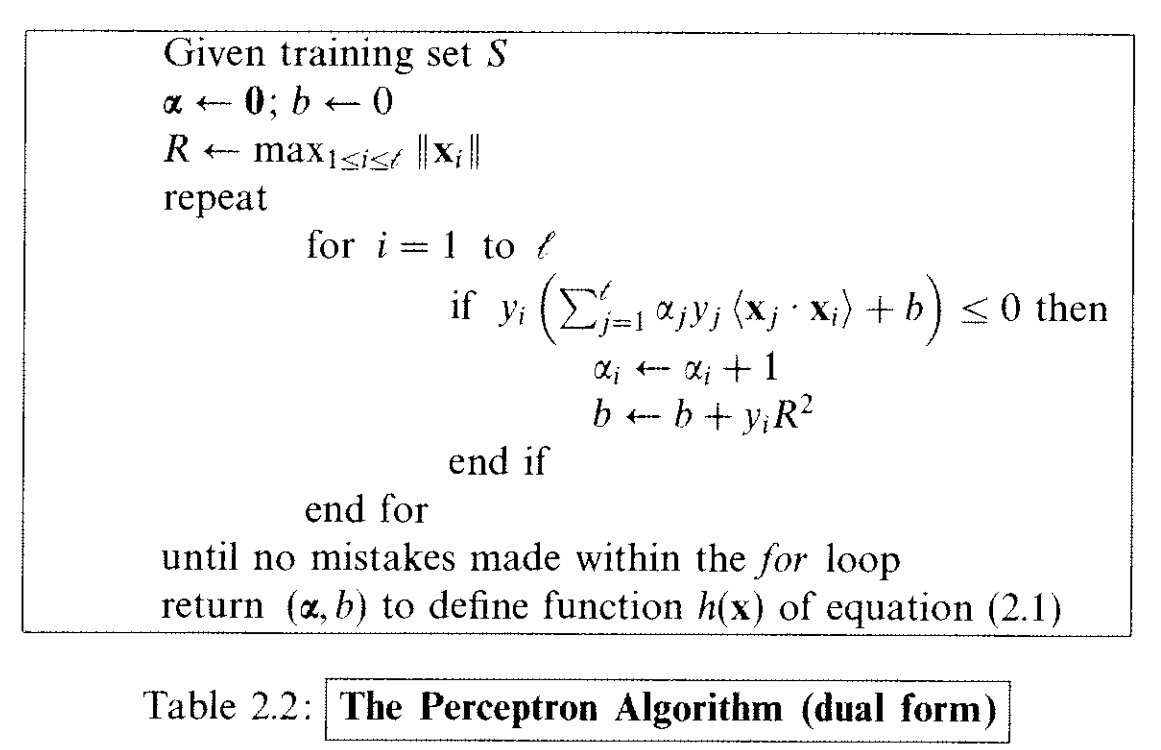
\includegraphics[width=0.7\linewidth]{pseudocodice_perceptron.png}
		\label{The Perceptron Algorithm (dual form)}
	\end{center}
	\subsection{KernelFunctions}
	La classe KernelFunctions fornisce tre metodi, uno per ogni tipologia di funzione kernel. 
	\begin{itemize}
		\item Linear kernel: prende in ingresso una matrice X e ritorna il prodotto scalare tra X e X trasposta.
		\item Polynomial kernel: prende in ingresso una matrice X, un paramentro c, che viene sommato al prodotto scalare come nel kernel lineare e un ultimo paramento d che definisce il grado del polinomio. 
		\item RBF kernel: prende in ingresso una matrice X e un parametro gamma e ritorna l'esponenziale della norma negativa moltiplicata per -gamma, il cui tutto è elevato al quadrato.
	\end{itemize}
    \subsection{MyDualPerceptron}
    La mia implementazione dell'algoritmo consiste nella classe MyDualPerceptron. Il costruttore prende in ingresso la tipologia di kernel che si vuole utilizzare, ovvero un numero: 1 per il kernel lineare, 2 per il kernel polinomiale e 3 per l'rbf kernel. Lo pseudocodice mostrato in Table 2.2 viene implementato nel metodo \textit{train()}, che prende in ingresso X, y, epochs. In particolare:
    \begin{itemize}
    	\item X: Porzione di data set, ovvero i dati che verrano utilizzati per addestrare il vettore alpha e il bias.
    	\item y: Porzione di data set, ovvero il vettore dei target di addestramento.
    	\item epochs: il numero di epoche(iterazioni) del ciclo for sul quale si vuole addestrare l'algoritmo.
    \end{itemize}
	Inoltre all'interno del metodo \textit{train()}, in base al tipo di kernel scelto dall'utente vengono mappati i dati di addestramento X e quindi creata la matrice K (nsamples,nsamples). Infine si utilizza un ciclo for per implementare il repeat dal quale si uscirà quando all'interno del ciclo for interno non ci saranno errori.
    Una volta eseguita la funzione di \textit{train()} che addestra i propri parametri alpha e b (bias), verrà chiamato il metodo \textit{predict()} che prende anche lui in ingresso X e y, i quali però non saranno uguali a quelli del \textit{train()}, ma saranno un'altra porzione di data set che viene utilizzata per testare l'accuracy dell'algoritmo nel predire i dati del target in output.
    \subsection{Main}
	Lo scopo principale della classe \textit{Main} è quello di leggere uno dei quattro data set messi a disposizione. Anche questi potranno essere scelti scrivendo un numero a scelta in particolare:
	\begin{itemize}
		\item 1: Breast Cancer Wisconsin (Diagnostic)
		\item 2: Adult
		\item 3: Heart Disease
		\item 4: Rice (Cammeo and Osmancik)
	\end{itemize}
	Da ogni data set vengono prese due porzioni: la prima X, che contiene tutte le colonne e le righe dei dati che servono all'algoritmo per dedurre il problema di classificazione binaria, mentre la seconda y, che contiene il vettore dei target. Il programma sfrutta: la libreria "numpy" per eseguire queste operazioni, in particolare i metodi \textit{iloc()} e \textit{where()} per, rispettivamente, prendere la porzione di dati interessa e modificare i valori interni in base a un vincolo per impostarli ad 1 o -1, e la libreria "sklearn" per i metodi \textit{train\_test\_split()} e \textit{accuracy()} per, rispettivamente, dividere X e y in un parte destinata all'addestramento e una parte invece destinata al test e al calcolo dell'accuracy della predizione finale.
	Successivamente vengono chiamati i metodi \textit{train()} e \textit{predict()} per l'esecuzione dell'addestramento dell'algoritmo e la predizione sui dati di test. Inoltre viene calcolato anche il tempo che l'algoritmo impiega a svolgere i propri metodi, grazie ad un ulteriore libreria "timeit". Infine viene calcolata l'accuracy con il metodo \textit{accuracy\_score()}
	\section{Analisi}
	All'interno di questa sezione viene analizzata l'accuracy dell'algoritmo DualPerceptron nel riuscire a predire i dati di test dei vari data set, utilizzando le varie tipologie di kernel. Di seguito viene mostrata una tabella con tutti i calcoli dell'accuracy.  
	Analizzando nel dettaglio i risultati, supponendo che la mole di dati di addestramento sia il 75\% e il 25\% di test, vediamo che:
	\begin{itemize}
		\item Breast Cancer Winsconsin (Diasgnostic): Questo data set contiene 30 colonne(n\_features) e 569 righe. Sia il kernel lineare che polinomiale non hanno ottimi risultati, mentre il kernel rbf riesce ad ottenere un risultato ottimo con un valore di gamma>=17.
		\item Adult: Questo è il più grande data set con 14 colonne e 32.581 righe, il cui scopo è quello di 
		\item Heart Disease: Questo data set contiene 13 colonne e 1026 righe, il cui scopo è 
		\item Rice (Cammeo and Osmancik): Questo data set contiene 7 colonne e 3810 righe, il cui scopo è 
	\end{itemize}
	\begin{table}[]
		\resizebox{\columnwidth}{!}{%
		\begin{tabular}{@{}l|l|l|l|@{}}
		\cmidrule(l){2-4}
		 &
		  Linear\_kernel &
		  Polynomial\_kernel &
		  RBF\_kernel \\ \midrule
		\multicolumn{1}{|l|}{\begin{tabular}[c]{@{}l@{}}Breast Cancer Wisconsin (Diagnostic)\\  con n\_features = 30\end{tabular}} &
		  37,8\% &
		  \begin{tabular}[c]{@{}l@{}}(c=1, d=2) : 43\%\\ (c=1, d=3) : 38\%\\ (c=1, d=n\_features) : 35\%\end{tabular} &
		  \begin{tabular}[c]{@{}l@{}}Con un valore di \\ gamma \textgreater{}= 17: 100\%\end{tabular} \\ \midrule
		\multicolumn{1}{|l|}{\begin{tabular}[c]{@{}l@{}}Adult \\ \\ con n\_features = 14\end{tabular}} &
		  \begin{tabular}[c]{@{}l@{}}100 \%\\ Time taken to train the data is 349s\\ Time taken to predict the target is 18s\end{tabular} &
		  \begin{tabular}[c]{@{}l@{}}Risultati con (c=1, d=2): 100\%\\                                         Time taken to train the data is 414s\\                                         Time taken to predict the target is 22s\\ Risultati con (c=1, d=3): Lasciato andare per 1 ora ma non ha dato risultato\end{tabular} &
		  Con gamma=1: \\ \midrule
		\multicolumn{1}{|l|}{\begin{tabular}[c]{@{}l@{}}Heart Disease\\ \\ con n\_features=13\end{tabular}} &
		  50\% &
		  \begin{tabular}[c]{@{}l@{}}Risultati con (c=1 e d=3): 51\% \\ Risultati con (c=1 e d=2): 52,5\%\end{tabular} &
		  \begin{tabular}[c]{@{}l@{}}Riassumendo con 1/100 \textless gamma \textless 1/20 risultati buoni\\ \\ tutti intorno all'85\%\end{tabular} \\ \midrule
		\multicolumn{1}{|l|}{\begin{tabular}[c]{@{}l@{}}Rice (Cammeo and Osmancik)\\ \\ con n\_features=7\end{tabular}} &
		  \begin{tabular}[c]{@{}l@{}}58\%\\ Time taken to train the data is 2371s\\ Time taken to predict the target is 0.26s\end{tabular} &
		  \begin{tabular}[c]{@{}l@{}}Risultati con (c=1, d=3): 42\%\\                                         Time taken to train the data is 2933s\\                                         Time taken to predict the target is 0.578s\end{tabular} &
		  Con gamma=1000: 100\% \\ \bottomrule
		\end{tabular}%
		}
	\end{table}
\end{document}